\section{引言}

\subsection{题目内容与分析}

  \begin{MainBox}[题目6:AI+物理实验]
    \textbf{目的:} 
    将AI技术与物理实验结合,实现物理现象的观察、物理参数的测量。

    \vspace{0.3cm}
    \textbf{要求:}
    \begin{enumerate}[leftmargin=*,nosep,label=\color{winered}\textbf{\arabic*.}]
        \item 设计实验方案(含原理);
        \item 制作实验装置,实现物理现象的观察与参数测量;
        \item 利用AI技术完成测量、数据处理或结果分析;  
        \item 讨论测量精度和不确定度。
    \end{enumerate}
  \end{MainBox}

通过分析,题目的要点是"将AI技术与物理实验结合"与"物理现象的观察、物理参数的测量",
所以本团队需要使用AI智能化的手段实现物理数据测量的精准度,同时设计一套实验装置实现上述功能,
以此来改进传统物理实验中存在的不足,实现将物理实验与AI技术的创新性结合,
同时平衡物理原理的严谨性与AI技术的实用性。

\subsection{背景探索}

随着人工智能技术的迅速发展,将AI技术应用于传统物理实验中已成为提高实验精度与效率的重要方向\textsuperscript{\cite{陈冲2025物理引导的深度学习研究综述}}。
本项目的背景基于两个方面的探索:传统物理实验中存在的问题与挑战,以及AI技术在科学测量领域的应用潜力。

传统物理实验教学中,单摆实验作为经典的力学现象观察与测量实验,长期存在精度低、操作繁琐等问题。
具体表现为:人工计时误差大,学生使用秒表记录往往受到反应延迟的影响;
重复测量负担重,为减小随机误差需要多次测量并计算平均值;实验条件限制严格,如必须保证小摆角条件等。
虽然目前教学中使用光电门计时、气垫导轨等设备可部分改善,但这些设备通常价格昂贵、体积大、操作复杂,不利于在基层学校普及。

在物理学科教育与研究中,计算机视觉技术已在多个领域展现出应用潜力。
如吴俊杰等人将摄像头和频闪截屏技术应用于单摆运动的研究\textsuperscript{\cite{WUJS200610016}},
张世功等人通过声卡采集光电门数据研究大幅度阻尼单摆的振动\textsuperscript{\cite{DWSL202206016}},
洪炎红等人将Tracker视频分析软件与中学物理教学整合\textsuperscript{\cite{WLTB201706010}}。
这些研究表明,信息化的实验测量方案不仅可以提高数据精度,还能降低实验门槛,促进物理教育的普及。
然而,这些研究成果仍然存在系列问题,如张世功等人的实验装置设备成本高、操作复杂、不易普及;
吴俊杰、洪炎红等人的实验装置设备体积大、不易携带,并且要保证在纯色背景下才能使用,限制了其应用场景。

目前针对单摆实验的 AI 辅助解决方案较少,特别是缺乏结合最新深度学习技术、易于操
作且成本低廉的综合系统。近年来,基于深度卷积神经网络(Convolutional Neural Network, CNN)的目标检测技术成为计算机视觉研究中
的一个热点,其中由Joseph Redmon等人在2015年首次提出的YOLO(You Only Look Once)目标检测算法,
通过单次查看即可完成对图像中物体的识别和定位,具有\textbf{速度快、准确率高、可解释性强和适用性广}等优点,
是当前目标检测领域最重要的代表之一\textsuperscript{\cite{jiang2022review}},这些特点使其特别适合实时物理实验测量,可以克服上述问题,具有良好的应用潜力。


\subsection{实验方案选择}
通过上述背景探索,本团队决定采用基于\textbf{YOLO目标检测算法}的单摆运动智能测量系统,以辅助传统单摆实验中重力加速度和阻尼系数的测量。本团队还将探讨该系统在物理实验教学中的应用效果,以推动人工智能与物理教育的深度融合。实验方案的框架如图\ref{实验方案框架}所示。


\begin{figure}[ht]
    \centering
    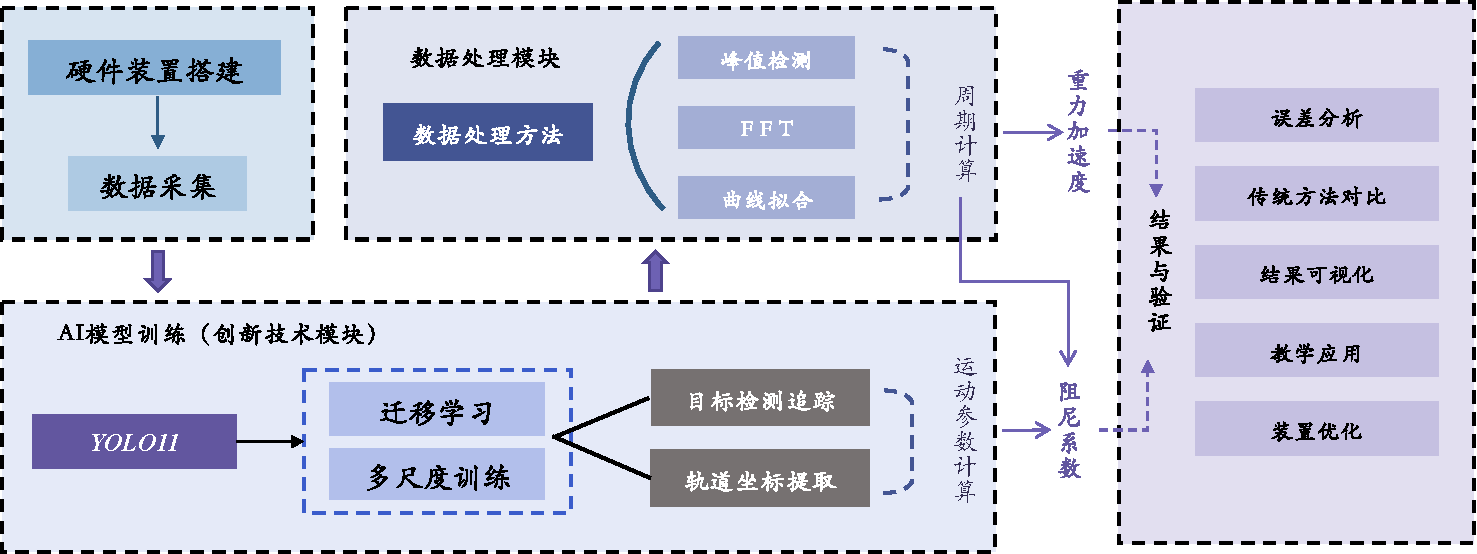
\includegraphics[width=1\textwidth]{figures/实验方案框架}
    \caption{实验方案框架}
    \label{实验方案框架}
\end{figure} 